\documentclass[aspectratio=169]{beamer}

% Theme: use metropolis if available (Overleaf usually has it), otherwise fall back.
\IfFileExists{beamerthememetropolis.sty}{
  \usetheme{metropolis}
}{
  \usetheme{Madrid}
}

\usepackage{graphicx}
\usepackage{booktabs}
\usepackage{amsmath}
\usepackage{amssymb}
\usepackage{hyperref}
\hypersetup{hidelinks}
\usepackage{adjustbox}
\usepackage{tikz}
\usetikzlibrary{arrows.meta,positioning,fit,calc}
\usepackage[round,authoryear]{natbib}

\graphicspath{{figures/}}
\setbeamersize{text margin left=0.7cm, text margin right=0.7cm}

% If metropolis is available, keep section pages minimal (we will show our own outline).
\IfFileExists{beamerthememetropolis.sty}{
  \metroset{sectionpage=none}
}{}

\AtBeginSection[]{
  \begin{frame}{Outline}
    \tableofcontents[currentsection]
  \end{frame}
}

% ----------------------------
% Helpers: fit & crop graphics
% ----------------------------
\newcommand{\FitGraphic}[2][]{%
  \includegraphics[width=\linewidth,height=0.78\textheight,keepaspectratio,#1]{#2}%
}
\newcommand{\FitGraphicSmall}[2][]{%
  \includegraphics[width=\linewidth,height=0.60\textheight,keepaspectratio,#1]{#2}%
}
\newcommand{\TrimGraphicSmall}[5]{%
  \FitGraphicSmall[trim=#2bp #3bp #4bp #5bp,clip]{#1}%
}
% Crop a 3-panel horizontal figure into one panel, then make it fill the column.
% Strategy: scale to 3*\linewidth first, then clip out 1/3 (so the visible part is ~\linewidth).
\newcommand{\ThirdLeft}[1]{%
  \adjustbox{width=\linewidth}{%
    \clipbox{0 0 {0.666\width} 0}{\includegraphics[width=3\linewidth]{#1}}%
  }%
}
\newcommand{\ThirdMid}[1]{%
  \adjustbox{width=\linewidth}{%
    \clipbox{{0.333\width} 0 {0.333\width} 0}{\includegraphics[width=3\linewidth]{#1}}%
  }%
}
\newcommand{\ThirdRight}[1]{%
  \adjustbox{width=\linewidth}{%
    \clipbox{{0.666\width} 0 0 0}{\includegraphics[width=3\linewidth]{#1}}%
  }%
}

\title{Physics-Informed Residual Diffusion for\\OD-Conditioned Trajectory Generation}
\author{Jinlin Wu}
\date{\today}

\begin{document}

\begin{frame}
  \titlepage
\end{frame}

\begin{frame}{Roadmap}
\begin{itemize}
  \item \textbf{Phase A (pipeline)}: strict, leakage-free dt-fixed protocol (split-first, train-only products).
  \item \textbf{Phase B (what we built)}: physics-informed \textbf{residual diffusion} + inference-time CFG; strong OD alignment and micro realism (best-of-$K$).
  \item \textbf{Phase C (what breaks)}: \textbf{Destination Gravity / topological collapse} --- detours are missing even with CFG.
  \item \textbf{Phase D (pivot)}: reframe as \textbf{trip-level decision + execution}; follow SOTA hierarchical planning.
\end{itemize}
\end{frame}

\begin{frame}{Task Definition}
\begin{itemize}
  \item Task: \textbf{KnownDestination} OD-conditioned trajectory generation (grid space, dt-fixed).
  \item Windows: history $H{=}8$, horizon $F{=}12$ (dt-fixed $\Delta t=30$s).
  \item Key challenge: \textbf{multi-modal trip-level decision + continuous execution}.
  \item Goals:
    \begin{itemize}
      \item \textbf{Coverage}: best-of-$K$ (oracle) ADE/FDE, distribution metrics (Fr\'echet/DTW).
      \item \textbf{Physical realism}: macroscopic motion (MSD curve, Rog).
    \end{itemize}
\end{itemize}
\end{frame}

\begin{frame}{Outline}
  \tableofcontents
\end{frame}

\section{Phase A: Pipeline}

\begin{frame}{Phase A (from raw data to strict pipeline)}
\textbf{Relation to previous stage:} starting from raw Shenzhen taxi GPS records, we need a reproducible pipeline before any model comparison.

\vspace{0.6em}
\textbf{Phase A objective:} eliminate ambiguity and leakage (dt, split, nav\_field source, normalization).

\vspace{0.6em}
\textbf{Phase A outputs:}
\begin{itemize}
  \item dt-fixed dataset ($\Delta t=30$s) and train/val/test splits
  \item train-only products: data\_stats.json (normalizer) + nav\_field.npz
  \item sanity checks (split overlap, metadata source, coordinate range, alignment)
\end{itemize}
\end{frame}

\begin{frame}{Phase A: Strict Data Contract (KISS)}
\begin{figure}
\centering
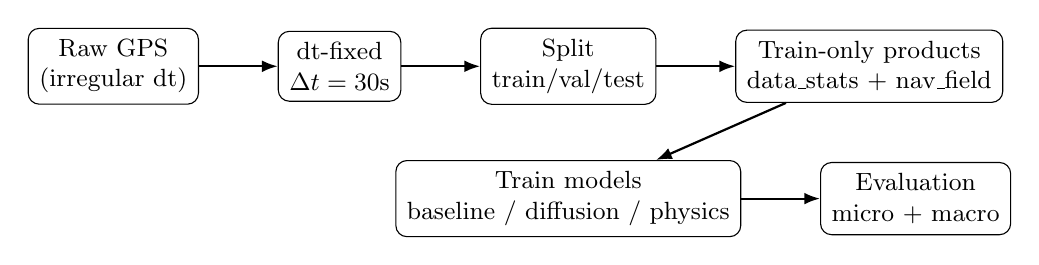
\begin{tikzpicture}[
  box/.style={draw, rounded corners, align=center, inner sep=4pt, font=\small},
  arrow/.style={-{Latex[length=2mm]}, thick},
  node distance=7mm and 10mm
]
  \node[box] (raw) {Raw GPS\\(irregular dt)};
  \node[box, right=of raw] (resample) {dt-fixed\\$\Delta t=30$s};
  \node[box, right=of resample] (split) {Split\\train/val/test};
  \node[box, right=of split] (products) {Train-only products\\data\_stats + nav\_field};
  \node[box, below=of split] (train) {Train models\\baseline / diffusion / physics};
  \node[box, right=of train] (eval) {Evaluation\\micro + macro};

  \draw[arrow] (raw) -- (resample);
  \draw[arrow] (resample) -- (split);
  \draw[arrow] (split) -- (products);
  \draw[arrow] (products) -- (train);
  \draw[arrow] (train) -- (eval);
\end{tikzpicture}
\caption*{\small Split-first, train-only products: prevents nav\_field/statistics leakage into val/test.}
\end{figure}
\end{frame}

\section{Phase B: Residual Diffusion (What Works)}

\begin{frame}{Our Method: Physics-Informed Residual Diffusion}
\begin{figure}
  \centering
  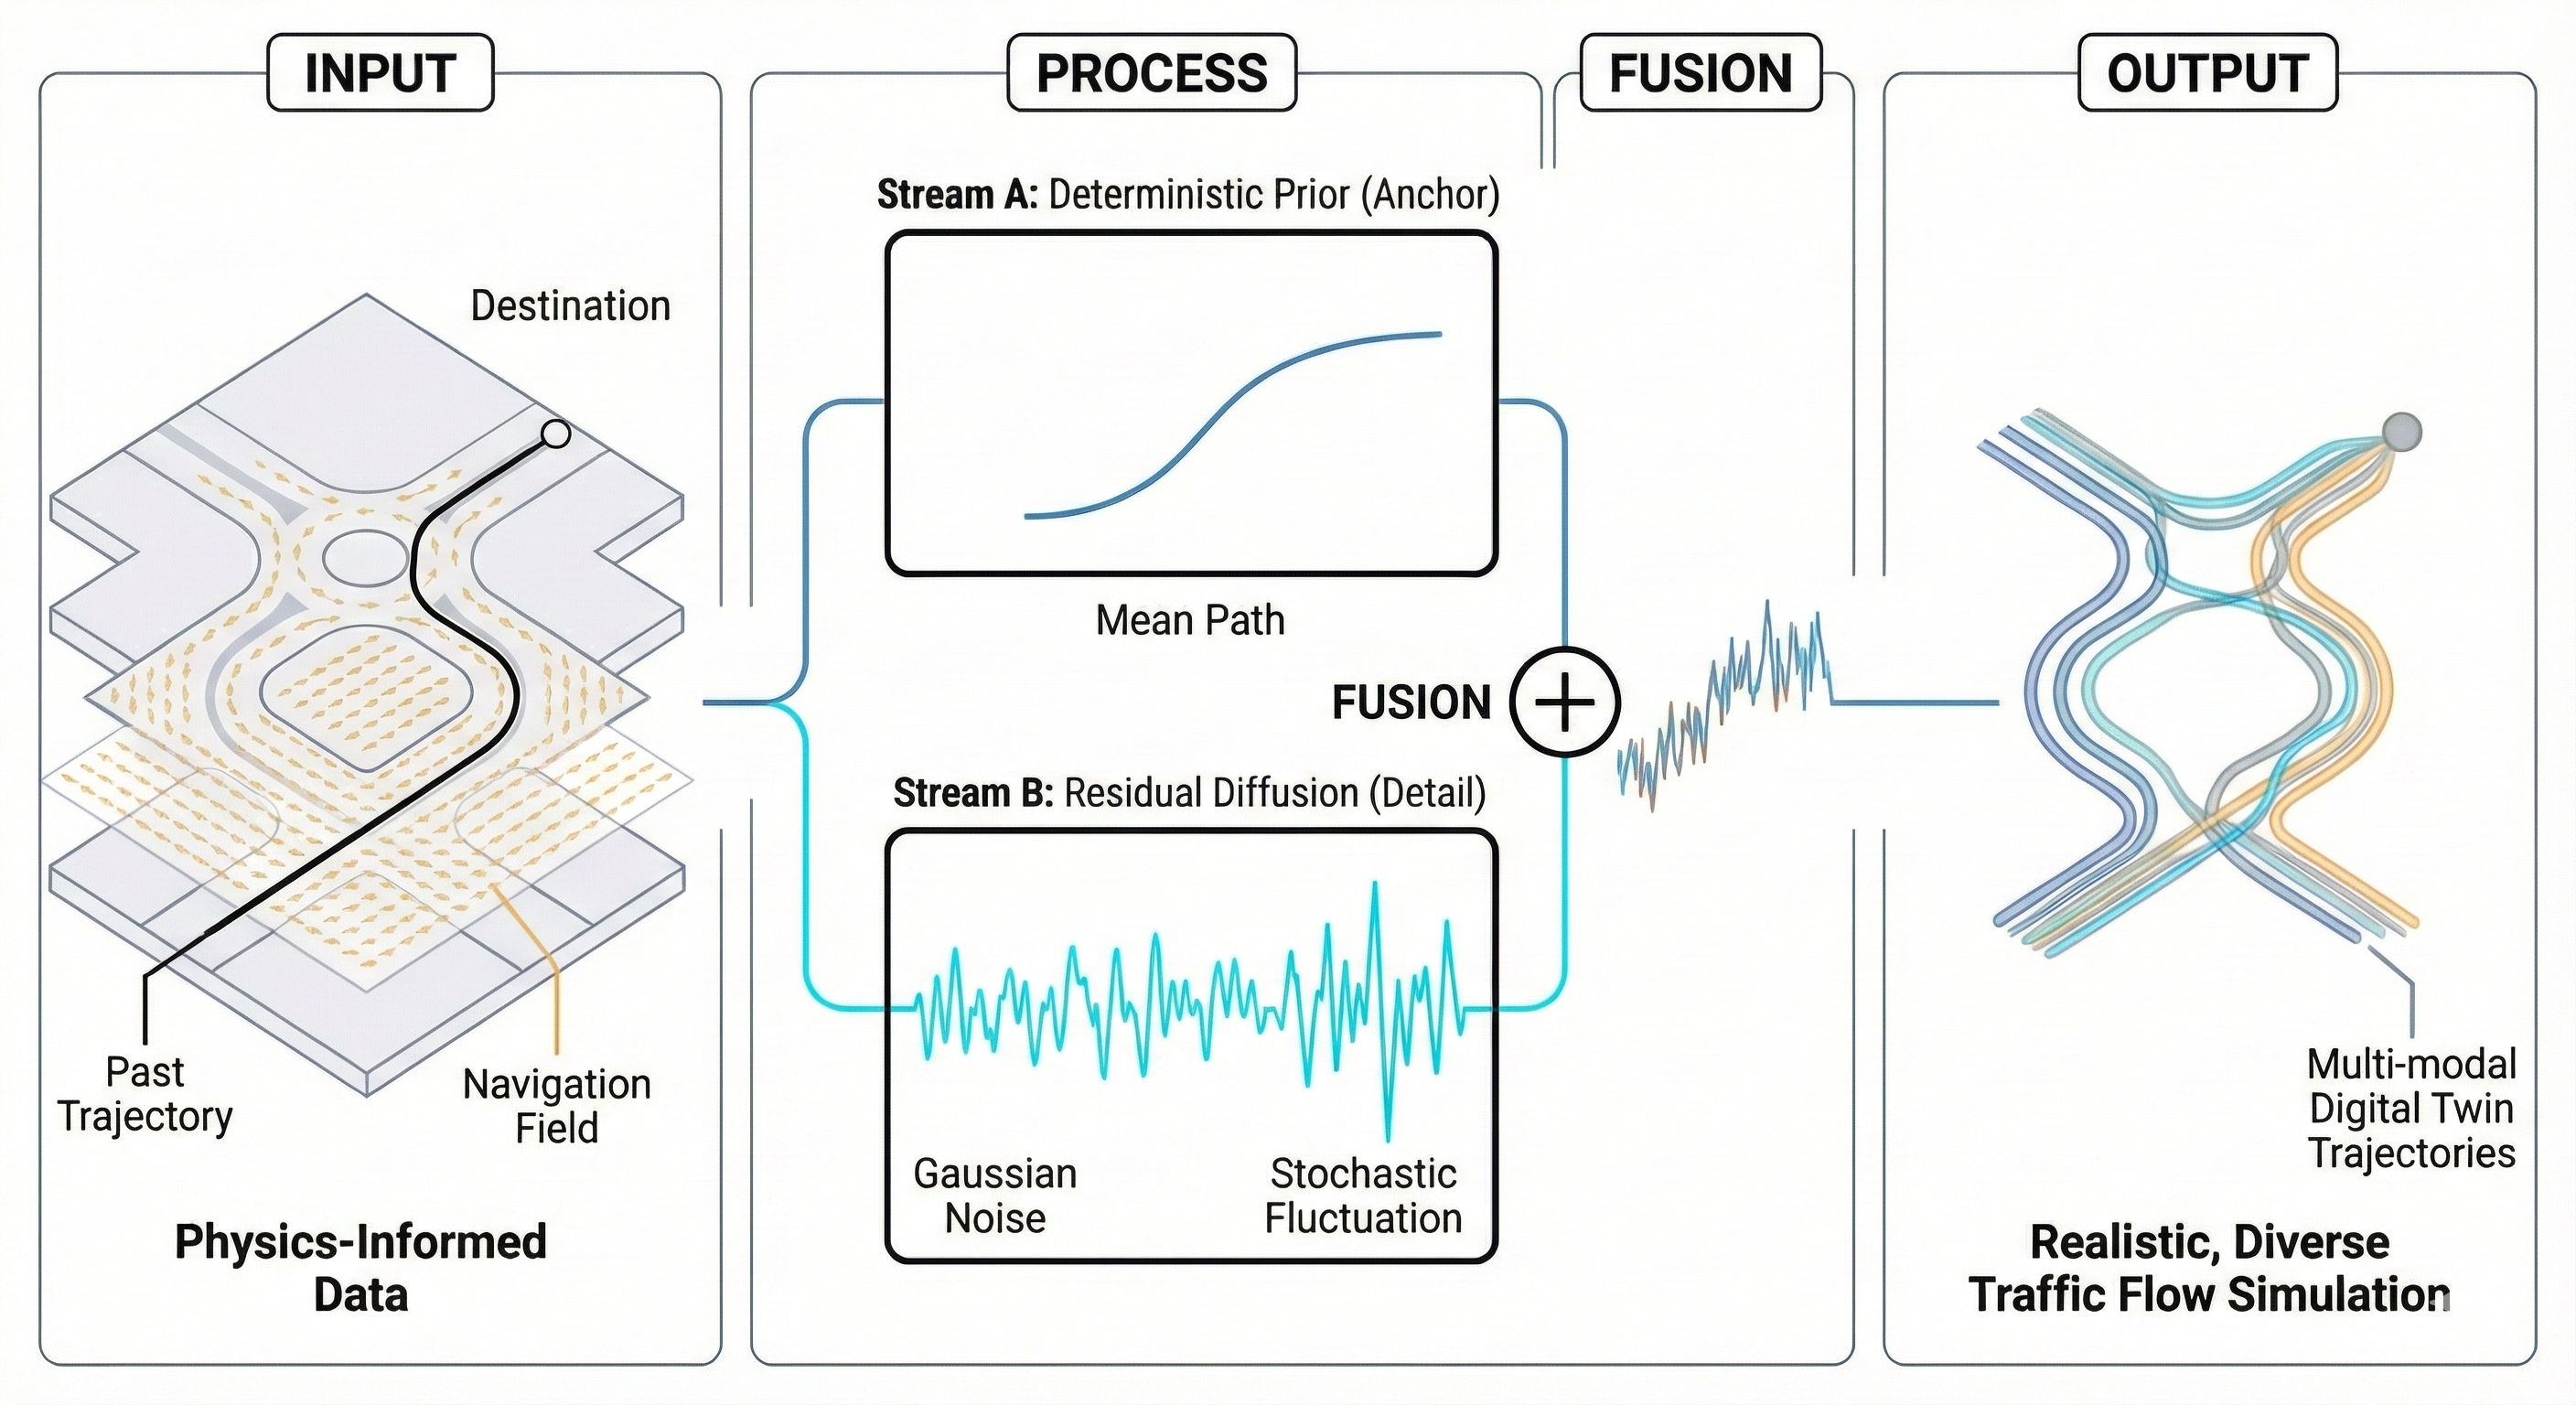
\includegraphics[width=\linewidth,height=0.78\textheight,keepaspectratio]{fig1_framework.png}
  \caption*{\small Deterministic prior anchors low-frequency scale; residual diffusion adds stochastic deviations (best-of-$K$) with nav\_field as local mean-flow prior.}
\end{figure}
\end{frame}

\begin{frame}{Macro: OD alignment in geographic space (Density, N=10k)}
\scriptsize\textbf{Reading guide:} GT density on the left; model density on the right (with GT contour). High sample size reveals corridor-level structure.
\vspace{0.2em}
\begin{figure}
  \centering
  \FitGraphic{stage_cfg_density10k/fig_geo_density.png}
  \caption*{\small Density map (log-count): model captures major corridors under OD conditioning.}
\end{figure}
\end{frame}

\begin{frame}{Micro: Multi-modal local execution (best-of-$K$)}
\scriptsize\textbf{Reading guide:} Left = deterministic prior (anchor), Mid/Right = residual diffusion samples under CFG ($K$ spaghetti). Residual adds local realism and diversity.
\vspace{0.2em}
\begin{figure}
  \centering
  \FitGraphic{stage_cfg/fig_geo_story_grid_top.png}
  \caption*{\small Case studies: residual diffusion produces diverse, physically plausible deviations around the prior.}
\end{figure}
\end{frame}

\begin{frame}{Physical Statistics (Validity): Speed/Turn/Accel + MSD}
\begin{figure}
  \centering
  \FitGraphic{physical_stats/fig_physical_stats_density10k.png}
  \caption*{\small Statistical consistency improves (JSD vs GT), but this alone does not guarantee correct trip-level topology.}
\end{figure}
\end{frame}

\section{Phase C: Failure Mode (Destination Gravity)}

\begin{frame}{The Defect: Destination Gravity / Premature Convergence}
\scriptsize\textbf{Observation:} regardless of Prior vs CFG2/CFG3, many predicted trajectories are ``pulled'' straight to the destination; GT often detours (e.g., to reach a highway entrance).
\vspace{0.2em}
\begin{figure}
  \centering
  \FitGraphic{stage_cfg/fig_geo_traj_overlay.png}
  \caption*{\small Trajectory overlays (Prior vs CFG2 vs CFG3): topology collapses towards a straight-to-goal path.}
\end{figure}
\end{frame}

\begin{frame}{Why CFG cannot create detours (first-principles view)}
\begin{itemize}
  \item Conditioning on destination is like a \textbf{potential well} at the goal: without intermediate barriers/anchors, trajectories follow the steepest descent (``straight-to-goal'').
  \item CFG scales this gradient at inference: it can change \textbf{tail/jitter/violations}, but it does \textbf{not} introduce new low-frequency topological modes.
  \item Oracle diagnostics (workstation runs): even with GT mid-way waypoint, turn-angle distribution does not recover $\Rightarrow$ detour modes are largely absent from the model support.
\end{itemize}
\end{frame}

\begin{frame}{Evidence snippet (validity metrics, dt-fixed)}
\scriptsize\textbf{Example (N=10k, K=1):} statistical consistency improves, but topology can still collapse.
\vspace{0.4em}
\begin{table}
  \centering
  \begin{tabular}{lrrrrr}
    \toprule
    Method & JSD$_{\text{Turn}}$ & JSD$_{\text{Speed}}$ & JSD$_{\text{Accel}}$ & DCV$_{\text{Speed}}$ & DCV$_{\text{Accel}}$ \\
    \midrule
    Prior & 0.0956 & 0.1423 & 0.2537 & 0.128\% & 0.002\% \\
    Ours (CFG2) & 0.0503 & 0.0727 & 0.0531 & 0.580\% & 0.733\% \\
    \bottomrule
  \end{tabular}
\end{table}
\vspace{-0.2em}
\begin{itemize}
  \item JSD improves: generated trajectories look more realistic statistically.
  \item But detour requires \textbf{low-frequency trip-level decisions}, not just local fluctuations.
\end{itemize}
\end{frame}

\section{Phase D: Pivot (Decision + Execution)}

\begin{frame}{Reframing: trip-level decision + continuous execution}
\begin{columns}[T,onlytextwidth]
  \begin{column}{0.56\linewidth}
    \begin{itemize}
      \item \textbf{Decision (macro)}: choose a route topology / a few waypoints (highway entrance, bridge, etc.).
      \item \textbf{Execution (micro)}: generate a smooth, feasible trajectory that follows the chosen plan.
      \item Our current end-to-end generator mixes them $\Rightarrow$ easy shortcut: ``straight-to-goal + jitter''.
    \end{itemize}
  \end{column}
  \begin{column}{0.42\linewidth}
    \begin{figure}
      \centering
      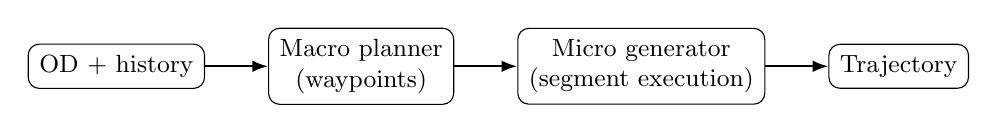
\begin{tikzpicture}[
        box/.style={draw, rounded corners, align=center, inner sep=4pt, font=\small},
        arrow/.style={-{Latex[length=2mm]}, thick},
        node distance=6mm and 8mm
      ]
        \node[box] (od) {OD + history};
        \node[box, right=of od] (macro) {Macro planner\\(waypoints)};
        \node[box, right=of macro] (micro) {Micro generator\\(segment execution)};
        \node[box, right=of micro] (traj) {Trajectory};
        \draw[arrow] (od) -- (macro);
        \draw[arrow] (macro) -- (micro);
        \draw[arrow] (micro) -- (traj);
      \end{tikzpicture}
      \caption*{\scriptsize Two-stage view: decision then execution.}
    \end{figure}
  \end{column}
\end{columns}
\end{frame}

\begin{frame}{How SOTA addresses Destination Gravity}
\begin{itemize}
  \item \textbf{Graph/Map-based diffusion} (e.g., road graph generation): topology is constrained by the road network, detours become natural turns at intersections.
  \item \textbf{Hierarchical / coarse-to-fine diffusion}: first generate a few waypoints (macro), then generate detailed paths between them (micro).
\end{itemize}
\vspace{0.4em}
\begin{table}
  \centering
  \begin{tabular}{lccc}
    \toprule
    Family & Topology validity & Data requirement & Engineering cost \\
    \midrule
    Graph/Map-based & strong & high (road graph) & high \\
    Hierarchical (waypoints) & strong detours & low (GPS only) & medium \\
    \bottomrule
  \end{tabular}
\end{table}
\end{frame}

\begin{frame}{Our next step: hierarchical decision + residual execution (KISS)}
\begin{itemize}
  \item \textbf{Macro stage (decision)}: predict a few waypoints (multi-modal) given OD + history.
  \item \textbf{Micro stage (execution)}: residual diffusion conditioned on waypoints to generate smooth segment trajectories.
  \item \textbf{Gate (avoid wrong turns)}: validate with detour-sensitive metrics (turn-angle distribution + low-frequency detour) + DCV.
  \item \textbf{Fallback}: only if hierarchical is insufficient, consider road graph / map constraints.
\end{itemize}
\end{frame}

\begin{frame}{References (selected)}
\scriptsize
\begin{thebibliography}{10}
\bibitem[Ho et~al.(2020)]{ho2020ddpm}
Ho, Jain, and Abbeel.
\newblock Denoising diffusion probabilistic models.
\newblock NeurIPS, 2020.

\bibitem[Song et~al.(2021)]{song2021sde}
Song, Meng, and Ermon.
\newblock Score-based generative modeling through stochastic differential equations.
\newblock ICLR, 2021.

\bibitem[Gupta et~al.(2018)]{gupta2018socialgan}
Gupta, Johnson, Fei-Fei, Savarese, and Alahi.
\newblock Social{GAN}: Socially acceptable trajectories with generative adversarial networks.
\newblock CVPR, 2018.

\bibitem[Salzmann et~al.(2020)]{salzmann2020trajectronpp}
Salzmann, Ivanovic, Chakravarty, and Pavone.
\newblock Trajectron++: Dynamically feasible trajectory forecasting with heterogeneous data.
\newblock ECCV, 2020.

\bibitem[DiffTraj(2023)]{difftraj2023}
DiffTraj.
\newblock SIGSPATIAL, 2023.

\bibitem[G-Diff(2024)]{gdiff2024}
G-Diff.
\newblock KDD, 2024.

\bibitem[Hierarchical Diffusion(2024)]{hierdiff2024}
Hierarchical diffusion for mobility (waypoint-first generation).
\newblock NeurIPS, 2024.
\end{thebibliography}
\end{frame}

\end{document}
